\begin{figure}[htb]
	\begin{center}
		\begin{minipage}[b]{0.9\linewidth}
			\centering
			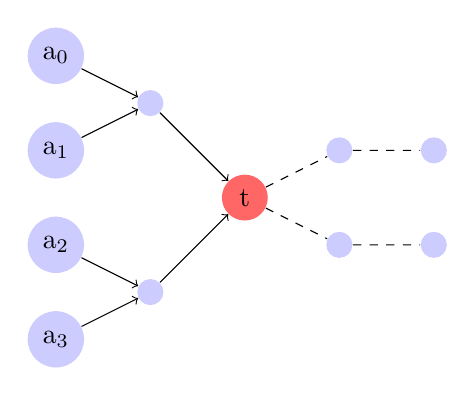
\begin{tikzpicture}
			  [scale=.6,auto=left,every node/.style={circle,fill=blue!20}]
			  \node (n11) at (1,7) {a$_0$};
			  \node (n12) at (1,5) {a$_1$};
			  \node (n2) at (3,6) { };
			  
	  		  \node (n31) at (1,3) {a$_2$};
	  		  \node (n32) at (1,1) {a$_3$};
			  \node (n4) at (3,2) { };
			  
			  \node[style={circle,fill=red!60}] (n5) at (5,4) {t};
			  
			  \node (n6) at (7,5) { };
			  \node (n7) at (7,3) { };
			  \node (n8) at (9,5) { };
			  \node (n9) at (9,3) { };
			  
			  \foreach \from/\to in {n11/n2,n12/n2,n2/n5,n31/n4,n32/n4,n4/n5}
			  \draw (\from) edge[->] (\to);
	
			  \foreach \from/\to in {n5/n6,n5/n7,n6/n8,n7/n9}
			  \draw (\from) edge[-,dashed] (\to);		  
			\end{tikzpicture}
			
			(a)\\
		\end{minipage}
		
		\bigskip
		\begin{minipage}[b]{0.9\linewidth}
			\centering
			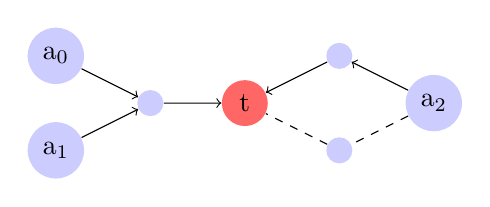
\begin{tikzpicture}
			  [scale=.6,auto=left,every node/.style={circle,fill=blue!20}]
			  \node (n11) at (1,3) {a$_0$};
			  \node (n12) at (1,1) {a$_1$};
			  \node (n2) at (3,2) { };
			  
	  		  \node (n3) at (9,2) {a$_2$};
			  \node (n41) at (7,3) { };
  			  \node (n42) at (7,1) { };
  			  
			  \node[style={circle,fill=red!60}] (n5) at (5,2) {t};
			  
			  \foreach \from/\to in {n11/n2,n12/n2,n2/n5,n3/n41,n41/n5}
			  \draw (\from) edge[->] (\to);
	
			  \foreach \from/\to in {n3/n42,n42/n5}
			  \draw (\from) edge[-,dashed] (\to);		  
			\end{tikzpicture}
			
			(b)
		\end{minipage}
	\end{center}
	\caption{\label{fig:error_phi}
	     Casos en los cuales la m\'etrica original pe\-na\-li\-za emboscadas
	     \'optimas. (a) Caso de no alcanzabilidad, dado que los agentes no
	     podr\'ian alcanzar a los nodos a la derecha de $t$ sin pasar por \'el.
	     (b) Caso de no existencia de mejor asignaci\'on posible, dado que
	     a pesar de contar con tres agentes, no es posible asignar caminos
	     que alcancen a $t$ a trav\'es de predecesores distintos a los agentes
	     $a_0$ y $a_1$.}
\end{figure}